\chapter{Hardware Implementation} \label{chap:hardware}
This chapter describes the hardware implementation, starting with a description of the \ac{ros} nodes in section \ref{sec:ros_nodes},
after which in section \ref{sec:ros_comms} the rost communication protocols are described.

\section{Overview}
The entire system in implemented using \ac{ros}, which is a system which, among other things, greatly simplifies the task of
communication between devices using various different communication protocols. This is achieved by sectioning all code into different
\ac{ros} nodes, where every node is treated a component in a large network. All ros nodes are joined together by the core node,
which is hosted at a set IP address on the network.

\newpage
\section{ROS Nodes} \label{sec:ros_nodes}
There are various ros nodes spread out across the base station, the Jetson Nano and the Teensy \ac{mcu}, figure \ref{fig:nodes} provides and overview
of the nodes and how they communicate with each other. Section \ref{sec:base_ros} and \ref{sec:on_board_ros} go into detail on the publishers and subscribers
on board the robot and on the base station. Figure \ref{fig:nodes} provides and overview of the \ac{ros} nodes and communication used to construct the system.
Further detail pertaining to communication using \ac{ros} is provided in section \ref{sec:ros_comms}.

\captionsetup[figure]{oneside,margin={0cm,0cm}}
\begin{figure}[h]
    \centering
    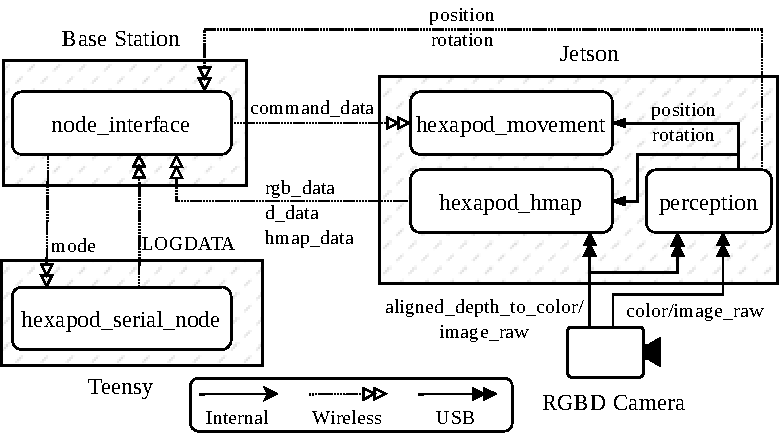
\includegraphics{Diagrams-Nodes.drawio.pdf}
    \caption{ROS nodes and communication.}
    \label{fig:nodes}
\end{figure}

\section{ROS communication} \label{sec:ros_comms}
    This section provides a detailed description of the \ac{ros} communication scheme used in the system as shown in figure \ref{fig:nodes}.
    \subsection{Base Station} \label{sec:base_ros}
        The base station wirelessly communicates with the robot to send commands and receive data.
        For a description of the base station publishers see table \ref{tab:base_pubs} and for its subscribers see \ref{tab:base_subs}. Table \ref{tab:data_types} describes
        data types used.
        \begin{table}[h]
            \centering
            \begin{tabularx}{\textwidth}{| l | l | X | l |}
                \hline
                \multicolumn{4}{|c|}{\textbf{Base Station Publishers}} \\ \hline
                \textbf{Name} & \textbf{Data Type} & \textbf{Description} & \textbf{Frequency} \\ \hline
                % walk\_dir & Description & Data Type & Frequency \\ \hline
                command\_data & HexapodCommands & Various robot command parameters. & On change \\ \hline
                mode & Int32 & Specifies the oporationg mode of the robot. & On change. \\ \hline
            \end{tabularx}
            \caption{Base station publishers}
            \label{tab:base_pubs}
        \end{table}
        
        The robot currently only has two operating modes, torque cutoff mode and walking mode. The torque cutoff mode is the initial mode the robot is in,
        while in this mode the leg servos disable all torque control, thus entering a relaxed state. In walking mode the robot walks in the commanded direction
        whilst optimising its foot positions according to the terrain. If the robot encounters a piece of terrain for which no optimisation can be found the
        human controller will have to adjust the walking direction from the base station.

        \begin{table}[h]
            \centering
            \begin{tabularx}{\textwidth}{| l | l | X |}
                \hline
                \multicolumn{3}{|c|}{\textbf{Base Station Subscribers}} \\ \hline
                \textbf{Name} & \textbf{Data Type} & \textbf{Description} \\ \hline
                % walk\_dir & Description & Data Type & Frequency \\ \hline
                rgb\_data & Image & The processed color image from the robot. \\ \hline
                d\_data & Image & The processed color depth from the robot. \\ \hline
                hmap\_data & Image & The heightmap generated on the robot. \\ \hline
                LOGDATA & String & General logs from the robot. \\ \hline
            \end{tabularx}
            \caption{Base station subscribers}
            \label{tab:base_subs}
        \end{table}
        
        \noindent
        The only subscribers present on the base station are the processed camera images, heightmap and logs. These are all used to provide a interface from where
        the operator can control the robot.

    \subsection{On Board} \label{sec:on_board_ros}
        The hexapod has two computational units on board, first the Jetson Nano, which handles all high level operations, including heightmap generation and scoring,
        foot optimisation, maintain a walking gait and localisation using ORB-SLAM3. Secondly a Teensy2.0 \ac{mcu} handles low level operations, including interpolating feet movement paths
        and servo control. 
        Table \ref{tab:jetson_pubs} to \ref{tab:teensy_subs} describe the \ac{ros} publishers and subscribers present on these two computational units.
        
        The camera data, heightmap data, position and rotation are published for display at the base station.
        While the effector targets are published for use on the Teensy to move the robot's feet to the optimised positions.
        \newpage
        \begin{table}[h]
            \centering
            \begin{tabularx}{\textwidth}{| l | l | X | l |}
                \hline
                \multicolumn{4}{|c|}{\textbf{Jetson Publishers}} \\ \hline
                \textbf{Name} & \textbf{Data Type} & \textbf{Description} & \textbf{Frequency} \\ \hline
                % walk\_dir & Description & Data Type & Frequency \\ \hline
                effector\_targets & EffectorTargets & Data indicating which feet to move where, and what type of interpolation to use. & On change\\ \hline
                rgb\_data & Image & The processed color image from the \ac{rgbd} camera. & 15Hz. \\ \hline
                d\_data & Image & The processed depth image from the \ac{rgbd} camera. & 15Hz. \\ \hline
                hmap\_data & Image & The heightmap generated on the robot. & 15Hz. \\ \hline
                position & Vector3 & The localised position of the robot & 15Hz \\ \hline
                rotation & Quat & The localised rotation of the robot & 15Hz \\ \hline
            \end{tabularx}
            \caption{Jetson publishers}
            \label{tab:jetson_pubs}
        \end{table}
        % \newpage
        \begin{table}[h]
            \centering
            \begin{tabularx}{\textwidth}{| l | l | X |}
                \hline
                \multicolumn{3}{|c|}{\textbf{Jetson Subscribers}} \\ \hline
                \textbf{Name}  & \textbf{Data Type} & \textbf{Description} \\ \hline
                % walk\_dir & Description & Data Type & Frequency \\ \hline
                command\_data & HexapodCommands & Operator commands. \\ \hline
                color/image\_raw & Image & Color image from the camera. \\ \hline
                aligned\_depth\_to\_color/image\_raw & Image & Depth image from the camera. \\ \hline
            \end{tabularx}
            \caption{Jetson subscribers}
            \label{tab:jetson_subs}
        \end{table}

        As can be seen from table \ref{tab:jetson_subs} the only subscribers required on the Jetson is the raw camera feed, 
        for constructing the heightmap, and the commands from the base station.

        Table \ref{tab:teensy_pubs} show that the Teensy publishes the current feet positions these are the positions calculated through \ac{fk}. Additionally
        log data is also published for use on the base station.
        \begin{table}[h]
            \begin{tabularx}{\textwidth}{| l | l | X | l |}
                \hline
                \multicolumn{4}{|c|}{\textbf{Teensy Publishers}} \\ \hline
                \textbf{Name} & \textbf{Data Type} & \textbf{Description} & \textbf{Frequency} \\ \hline
                LOGDATA & String & General logs. & 10Hz \\ \hline
                effector\_current\_position & Eigen::Vector3d & Current feet positions. & 10Hz \\ \hline
            \end{tabularx}
            \caption{Teensy publishers}
            \label{tab:teensy_pubs}
        \end{table}
        \begin{table}[h]
            \centering
            \begin{tabularx}{\textwidth}{| l | l | X |}
                \hline
                \multicolumn{3}{|c|}{\textbf{Teensy subscribers}} \\ \hline
                \textbf{Name} & \textbf{Data Type} & \textbf{Description} \\ \hline
                % walk\_dir & Description & Data Type & Frequency \\ \hline
                command\_data & HexapodCommands & The color image from the \ac{rgbd} camera. \\ \hline
                effector\_targets & EffectorTargets & Data indicating which feet to move where, and what type of interpolation to use.\\ \hline
                mode & Int32 & Receives mode data from the base station \\ \hline
            \end{tabularx}
            \caption{Teensy subscribers}
            \label{tab:teensy_subs}
        \end{table}

        Lastly, from table \ref{tab:teensy_subs} it can be seen that the Teensy subscribes to the command data, effector targets and mode.
        The walking speed component from the command data is used to set the rotational rate of the servos, as discussed in section \ref{sec:ang_rate}.
        The effector targets are used to interpolate a curve for the feet to move along, as described in section \ref{sec:arc_generation}. The mode is required
        as some modes could integrate directly with the servo control, namely the torque cutoff mode.

    \newpage
    \subsection{ROS Data Types}
        Various custom \ac{ros} data types are defined to assist with communication, these data types are described in table \ref{tab:data_types}.
        \begin{table}[h]
            \centering
            \begin{tabularx}{\textwidth}{| l | p{\widthof{float32\([2]\) walk\_dir}} | X |}
                \hline
                \textbf{Name} & \textbf{Type Definition} & \textbf{Description} \\ \hline
                % walk\_dir & Description & Data Type & Frequency \\ \hline
                Vector3 & float\([3]\) data. & A vector in 3D space.  \\
                \hline
                EffectorTargets & Vector3\([6]\) targets \newline 
                                bool\([6]\) swinging. & Data describing the targets of the robot's feet and which feet are swinging. \\
                \hline
                HexapodCommands & float32\([2]\) walk\_dir \newline
                                float32 speed \newline
                                float32 height & Data packet containing various command parameters for the robot. \\
                \hline
            \end{tabularx}
            \caption{\ac{ros} data type descriptions}
            \label{tab:data_types}
        \end{table}